\section{Рабочий проект}
\subsection{Описание компонентов и классов программы}
\subsubsection{Описание классов сервиса аутентификации}
\paragraph{Описание класса AuthController}

Данный контроллер отвечает за регистрацию и авторизацию пользователей, а также за инвалидацию токенов, выданных пользователю, после выхода из приложения.

Описание полей и методов класса AuthController представлено в таблицах \ref{classAuthFields:table} и \ref{classAuthMethods:table} соответственно.

\renewcommand{\arraystretch}{0.8} % уменьшение расстояний до сетки таблицы
\begin{xltabular}{\textwidth}{|X|p{2.5cm}|>{\setlength{\baselineskip}{0.7\baselineskip}}p{4.83cm}|>{\setlength{\baselineskip}{0.7\baselineskip}}p{4.85cm}|}
	\caption{Описание полей класса AuthController}\label{classAuthFields:table}
	\hline \centrow \setlength{\baselineskip}{0.7\baselineskip} Название поля & \centrow \setlength{\baselineskip}{0.7\baselineskip} Область видимости & \centrow Тип данных & \centrow Описание \\
	\hline \centrow 1 & \centrow 2 & \centrow 3 & \centrow 4\\ \hline
	\endfirsthead
	\continuecaption{Продолжение таблицы \ref{classAuthFields:table}}
	\hline \centrow 1 & \centrow 2 & \centrow 3 & \centrow 4\\ \hline
	\finishhead
	dbContext & private & ChatDbContext & Контекст базы данных приложения\\
	\hline jwtService & private & JwtService & Сервис, отвечающий за работу с jwt-токенами \\
\end{xltabular}
\renewcommand{\arraystretch}{1.0}

\begin{xltabular}{\textwidth}{|X|p{2.5cm}|>{\setlength{\baselineskip}{0.7\baselineskip}}p{4.83cm}|}
	\caption{Описание методов класса AuthController}\label{classAuthMethods:table}
	\hline \centrow Название поля & \centrow Область видимости & \centrow Описание \\ \hline \centrow 1 & \centrow 2 & \centrow 3\\
	\hline 
	\endfirsthead
	\continuecaption{Продолжение таблицы \ref{classAuthMethods:table}}
	\hline \centrow 1 & \centrow 2 & \centrow 3 \\ \hline
	\finishhead
	SignUp & public & Действие контроллера, отвечающее за регистрацию пользователей \\ \hline
	SignIn & public & Действие контроллера, отвечающее за авторизацию пользователей \\ \hline
\end{xltabular}

\renewcommand{\arraystretch}{1.0}

\paragraph{Описание класса TokensController}

Данный коетроллер отвечает за выдачу токенов чатов и обновление токенов доступа приложения.

Описание полей и методов класса TokensController представлено в таблицах \ref{classTokensFields:table} и \ref{classTokensMethods:table} соответственно.

\renewcommand{\arraystretch}{0.8} % уменьшение расстояний до сетки таблицы
\begin{xltabular}{\textwidth}{|X|p{2.5cm}|>{\setlength{\baselineskip}{0.7\baselineskip}}p{4.83cm}|>{\setlength{\baselineskip}{0.7\baselineskip}}p{4.85cm}|}
	\caption{Описание полей класса AuthController}\label{classTokensFields:table}
	\hline \centrow \setlength{\baselineskip}{0.7\baselineskip} Название поля & \centrow \setlength{\baselineskip}{0.7\baselineskip} Область видимости & \centrow Тип данных & \centrow Описание \\
	\hline \centrow 1 & \centrow 2 & \centrow 3 & \centrow 4\\ \hline
	\endfirsthead
	\continuecaption{Продолжение таблицы \ref{classTokensFields:table}}
	\hline \centrow 1 & \centrow 2 & \centrow 3 & \centrow 4\\ \hline
	\finishhead
	dbContext & private & ChatDbContext & Контекст базы данных приложения\\
	\hline jwtService & private & JwtService & Сервис, отвечающий за работу с jwt-токенами \\
\end{xltabular}
\renewcommand{\arraystretch}{1.0}

\begin{xltabular}{\textwidth}{|X|p{2.5cm}|>{\setlength{\baselineskip}{0.7\baselineskip}}p{4.83cm}|}
	\caption{Описание методов класса AuthController}\label{classTokensMethods:table}
	\hline \centrow Название поля & \centrow Область видимости & \centrow Описание \\ \hline \centrow 1 & \centrow 2 & \centrow 3\\
	\hline 
	\endfirsthead
	\continuecaption{Продолжение таблицы \ref{classTokensMethods:table}}
	\hline \centrow 1 & \centrow 2 & \centrow 3 \\ \hline
	\finishhead
	GetChatToken & public & Действие контроллера, отвечающее за выдачу токенов конкретного чата \\ \hline
	RefreshAccessToken & public & Действие контроллера, отвечающее за обновление токена доступа \\ \hline
	RefreshChatToken & public & Действие контроллера, отвечающее за обновление токенов чатов \\ \hline
\end{xltabular}

\renewcommand{\arraystretch}{1.0}

\paragraph{Описание класса JwtService}

Данный класс отвечает за непосредственную генерацию jwt-токенов. Данный класс используется в контроллере регистрации и авторизации и контроллере токенов.

Описание полей и методов класса JwtService представлено в таблицах \ref{classJwtFields:table} и \ref{classJwtMethods:table} соответственно.

\renewcommand{\arraystretch}{0.8} % уменьшение расстояний до сетки таблицы
\begin{xltabular}{\textwidth}{|X|p{2.5cm}|>{\setlength{\baselineskip}{0.7\baselineskip}}p{4.83cm}|>{\setlength{\baselineskip}{0.7\baselineskip}}p{4.85cm}|}
	\caption{Описание полей класса JwtService}\label{classJwtFields:table}
	\hline \centrow \setlength{\baselineskip}{0.7\baselineskip} Название поля & \centrow \setlength{\baselineskip}{0.7\baselineskip} Область видимости & \centrow Тип данных & \centrow Описание \\
	\hline \centrow 1 & \centrow 2 & \centrow 3 & \centrow 4\\ \hline
	\endfirsthead
	\continuecaption{Продолжение таблицы \ref{classJwtFields:table}}
	\hline \centrow 1 & \centrow 2 & \centrow 3 & \centrow 4\\ \hline
	\finishhead
	configuration & private & IConfiguration & Данное поле обеспечивает к конфигурации приложения\\
\end{xltabular}
\renewcommand{\arraystretch}{1.0}

\begin{xltabular}{\textwidth}{|X|p{2.5cm}|>{\setlength{\baselineskip}{0.7\baselineskip}}p{4.83cm}|}
	\caption{Описание методов класса JwtService}\label{classJwtMethods:table}
	\hline \centrow Название поля & \centrow Область видимости & \centrow Описание \\ \hline \centrow 1 & \centrow 2 & \centrow 3\\
	\hline 
	\endfirsthead
	\continuecaption{Продолжение таблицы \ref{classJwtMethods:table}}
	\hline \centrow 1 & \centrow 2 & \centrow 3 \\ \hline
	\finishhead
	GetAccessToken & public & Метод, отвечающий за генерацию токенов доступа \\ \hline
	GetRefreshToken & public & Метод, отвечающий за генерацию токенов обновления \\ \hline
	GetChatToken & public & Метод, отвечающий за генерацию токенов чатов \\ \hline
\end{xltabular}

\renewcommand{\arraystretch}{1.0}

\subsubsection{Описание классов приложения}

\paragraph{Описание класса ChatController}

Данный контроллер отвечает за функционал конкретного чата, т. е. отправку сообщений в этот чат, добавление и удаление пользователей, приглашение пользователей в чат и т.д.

Описание полей и методов класса ChatController представлено в таблицах \ref{classChatFields:table} и \ref{classChatMethods:table} соответственно.

\renewcommand{\arraystretch}{0.8} % уменьшение расстояний до сетки таблицы
\begin{xltabular}{\textwidth}{|X|p{2.5cm}|>{\setlength{\baselineskip}{0.7\baselineskip}}p{4.83cm}|>{\setlength{\baselineskip}{0.7\baselineskip}}p{4.85cm}|}
	\caption{Описание полей класса ChatController}\label{classChatFields:table}
	\hline \centrow \setlength{\baselineskip}{0.7\baselineskip} Название поля & \centrow \setlength{\baselineskip}{0.7\baselineskip} Область видимости & \centrow Тип данных & \centrow Описание \\
	\hline \centrow 1 & \centrow 2 & \centrow 3 & \centrow 4\\ \hline
	\endfirsthead
	\continuecaption{Продолжение таблицы \ref{classChatFields:table}}
	\hline \centrow 1 & \centrow 2 & \centrow 3 & \centrow 4\\ \hline
	\finishhead
	dbContext & private & ChatDbContext & Контекст базы данных приложения\\
	\hline hubContext & private & IHubContext<ChatHub> & Контекст хаба чатов, для возможности рассылки обновлений пользователям чата в реальном времени \\
\end{xltabular}
\renewcommand{\arraystretch}{1.0}

\begin{xltabular}{\textwidth}{|X|p{2.5cm}|>{\setlength{\baselineskip}{0.7\baselineskip}}p{4.83cm}|}
	\caption{Описание методов класса AuthController}\label{classChatMethods:table}
	\hline \centrow Название поля & \centrow Область видимости & \centrow Описание \\ \hline \centrow 1 & \centrow 2 & \centrow 3\\
	\hline 
	\endfirsthead
	\continuecaption{Продолжение таблицы \ref{classChatMethods:table}}
	\hline \centrow 1 & \centrow 2 & \centrow 3 \\ \hline
	\finishhead
	SendMessage & public & Метод, отвечающий за отправку сообщения в чат \\ \hline
	DeleteMessage & public & Метод, отвечающий за удаление сообщения из чата \\ \hline
	GetMessages & public & Метод, возвращающий все сообщения чата \\ \hline
	GetUsers & public & Метод, возвращающий всех пользователей в чате \\ \hline
	DeleteUser & public & Метод, отвечающий за удаление пользователя из чата \\ \hline
\end{xltabular}

\renewcommand{\arraystretch}{1.0}

\paragraph{Описание класса ChatsController}

Данный контроллер отвечает за управление всеми чатами, т. е. создание нового чата, удаление чата, обновление информации о чате и т.д.

Описание полей и методов класса ChastController представлено в таблицах \ref{classChatsFields:table} и \ref{classChatsMethods:table} соответственно.

\renewcommand{\arraystretch}{0.8} % уменьшение расстояний до сетки таблицы
\begin{xltabular}{\textwidth}{|X|p{2.5cm}|>{\setlength{\baselineskip}{0.7\baselineskip}}p{4.83cm}|>{\setlength{\baselineskip}{0.7\baselineskip}}p{4.85cm}|}
	\caption{Описание полей класса ChatsController}\label{classChatsFields:table}
	\hline \centrow \setlength{\baselineskip}{0.7\baselineskip} Название поля & \centrow \setlength{\baselineskip}{0.7\baselineskip} Область видимости & \centrow Тип данных & \centrow Описание \\
	\hline \centrow 1 & \centrow 2 & \centrow 3 & \centrow 4\\ \hline
	\endfirsthead
	\continuecaption{Продолжение таблицы \ref{classChatsFields:table}}
	\hline \centrow 1 & \centrow 2 & \centrow 3 & \centrow 4\\ \hline
	\finishhead
	dbContext & private & ChatDbContext & Контекст базы данных приложения \\
\end{xltabular}
\renewcommand{\arraystretch}{1.0}

\begin{xltabular}{\textwidth}{|X|p{2.5cm}|>{\setlength{\baselineskip}{0.7\baselineskip}}p{4.83cm}|}
	\caption{Описание методов класса ChatsController}\label{classChatsMethods:table}
	\hline \centrow Название поля & \centrow Область видимости & \centrow Описание \\ \hline \centrow 1 & \centrow 2 & \centrow 3\\
	\hline 
	\endfirsthead
	\continuecaption{Продолжение таблицы \ref{classChatsMethods:table}}
	\hline \centrow 1 & \centrow 2 & \centrow 3 \\ \hline
	\finishhead
	AddNewChat & public & Метод, отвечающий за добавление нового чата \\ \hline
	DeleteChat & public & Метод, отвечающий за удаление чата \\ \hline
	UpdateChat & public & Метод, отвечающий за обновлении информации о чате \\ \hline
\end{xltabular}

\renewcommand{\arraystretch}{1.0}

\paragraph{Описание класса UserController}

Данный контроллер отвечает за доступ к данным конкретного пользователя. 

Описание полей и методов класса UserController представлено в таблицах \ref{classUserFields:table} и \ref{classUserMethods:table} соответственно.

\renewcommand{\arraystretch}{0.8} % уменьшение расстояний до сетки таблицы
\begin{xltabular}{\textwidth}{|X|p{2.5cm}|>{\setlength{\baselineskip}{0.7\baselineskip}}p{4.83cm}|>{\setlength{\baselineskip}{0.7\baselineskip}}p{4.85cm}|}
	\caption{Описание полей класса UserController}\label{classUserFields:table}
	\hline \centrow \setlength{\baselineskip}{0.7\baselineskip} Название поля & \centrow \setlength{\baselineskip}{0.7\baselineskip} Область видимости & \centrow Тип данных & \centrow Описание \\
	\hline \centrow 1 & \centrow 2 & \centrow 3 & \centrow 4\\ \hline
	\endfirsthead
	\continuecaption{Продолжение таблицы \ref{classUserFields:table}}
	\hline \centrow 1 & \centrow 2 & \centrow 3 & \centrow 4\\ \hline
	\finishhead
	dbContext & private & ChatDbContext & Контекст базы данных приложения \\
\end{xltabular}
\renewcommand{\arraystretch}{1.0}

\begin{xltabular}{\textwidth}{|X|p{2.5cm}|>{\setlength{\baselineskip}{0.7\baselineskip}}p{4.83cm}|}
	\caption{Описание методов класса ChatsController}\label{classUserMethods:table}
	\hline \centrow Название поля & \centrow Область видимости & \centrow Описание \\ \hline \centrow 1 & \centrow 2 & \centrow 3\\
	\hline 
	\endfirsthead
	\continuecaption{Продолжение таблицы \ref{classUserMethods:table}}
	\hline \centrow 1 & \centrow 2 & \centrow 3 \\ \hline
	\finishhead
	GetUserChats & public & Метод, отвечающий за получение чатов, в которых состоит пользователь \\ \hline
	GetUserInvitations & public & Метод, отвечающий за получение приглашений пользователя в чаты \\ \hline
\end{xltabular}

\renewcommand{\arraystretch}{1.0}

\paragraph{Описание класса UsersController}

Данный контроллер отвечает за управление всем пользователями, т. е. получение информации о пользователе, удаление пользователя из приложения и т. д.

Описание полей и методов класса UsersController представлено в таблицах \ref{classUsersFields:table} и \ref{classUsersMethods:table} соответственно.

\renewcommand{\arraystretch}{0.8} % уменьшение расстояний до сетки таблицы
\begin{xltabular}{\textwidth}{|X|p{2.5cm}|>{\setlength{\baselineskip}{0.7\baselineskip}}p{4.83cm}|>{\setlength{\baselineskip}{0.7\baselineskip}}p{4.85cm}|}
	\caption{Описание полей класса UserController}\label{classUsersFields:table}
	\hline \centrow \setlength{\baselineskip}{0.7\baselineskip} Название поля & \centrow \setlength{\baselineskip}{0.7\baselineskip} Область видимости & \centrow Тип данных & \centrow Описание \\
	\hline \centrow 1 & \centrow 2 & \centrow 3 & \centrow 4\\ \hline
	\endfirsthead
	\continuecaption{Продолжение таблицы \ref{classUsersFields:table}}
	\hline \centrow 1 & \centrow 2 & \centrow 3 & \centrow 4\\ \hline
	\finishhead
	dbContext & private & ChatDbContext & Контекст базы данных приложения \\
\end{xltabular}
\renewcommand{\arraystretch}{1.0}

\begin{xltabular}{\textwidth}{|X|p{2.5cm}|>{\setlength{\baselineskip}{0.7\baselineskip}}p{4.83cm}|}
	\caption{Описание методов класса ChatsController}\label{classUsersMethods:table}
	\hline \centrow Название поля & \centrow Область видимости & \centrow Описание \\ \hline \centrow 1 & \centrow 2 & \centrow 3\\
	\hline 
	\endfirsthead
	\continuecaption{Продолжение таблицы \ref{classUsersMethods:table}}
	\hline \centrow 1 & \centrow 2 & \centrow 3 \\ \hline
	\finishhead
	DeleteUser & public & Метод, отвечающий за удаление пользователя \\ \hline
	UpdateUser & public & Метод, отвечающий за обновление данных пользователя \\ \hline
\end{xltabular}

\renewcommand{\arraystretch}{1.0}

\subsection{Тестирование программной системы}

\subsubsection{Модульное тестирование}

Для проверки работоспособности отдельных модулей программной системы было проведено модульное тестирование.

Модульное тестирование — это метод проверки программного обеспечения, при котором отдельные модули или компоненты тестируются независимо от остальных частей системы. Основная цель модульных тестов — убедиться в корректности работы каждого отдельного блока кода программы. Тесты позволяют выявлять ошибки и недочеты на ранних стадиях разработки, обеспечивая уверенность в стабильности и надежности программного продукта. Автоматизированные модульные тесты выполняются быстро и могут быть запущены в любой среде, что делает процесс тестирования более эффективным и повышает общее качество кода.

На рисунке \ref{unitGetChatToken:image} представлен модульный тест метода GetChatToken класса TokensController.

\begin{figure}[H]
	\begin{lstlisting}
		[Fact]
		public async Task GetChatToken_ReturnsUnauthorized_WhenUserChatNotFound()
		{
			// Arrange
			int userId = 1;
			int chatId = 1;
			var user = new User { UserId = userId };
			
			dbContextMock.Setup(db => db.Users.FindAsync(userId)).ReturnsAsync(user);
			dbContextMock.Setup(db => db.UsersInChats.SingleOrDefault(It.IsAny<Func<UsersInChat, bool>>())).Returns((UsersInChat)null);
			
			var controller = new TokensController(dbContextMock.Object, jwtServiceMock.Object);
			controller.ControllerContext.HttpContext = httpContext;
			
			// Act
			var result = await controller.GetChatToken(chatId);
			
			// Assert
			Assert.IsType<UnauthorizedResult>(result);
		}
	\end{lstlisting}
	\caption{Модульный тест метода GetChatToken класса TokensController}
	\label{unitGetChatToken:image}
\end{figure}

На рисунке \ref{unitRefreshAccessToken:image} представлен модульный тест метода RefreshAccessToken класса TokensController.

\begin{figure}[H]
	\begin{lstlisting}
		[Fact]
		public async Task RefreshAccessToken_ReturnsNoContentResult()
		{
			// Arrange
			int userId = 1;
			var user = new User { UserId = userId, Login = "testuser" };
			
			dbContextMock.Setup(db => db.Users.FindAsync(userId)).ReturnsAsync(user);
			
			string fakeToken = "Bearer fakeToken";
			jwtServiceMock.Setup(jwt => jwt.GetAccessToken(userId, user.Login)).Returns(fakeToken);
			
			var controller = new TokensController(dbContextMock.Object, jwtServiceMock.Object);
			controller.ControllerContext.HttpContext = httpContext;
			
			// Act
			var result = await controller.RefreshAccessToken();
			
			// Assert
			var noContentResult = Assert.IsType<NoContentResult>(result);
			Assert.Equal(fakeToken, httpContext.Response.Headers["Authorization"]);
		}
	\end{lstlisting}
	\caption{Модульный тест метода RefreshAccessToken класса TokensController}
	\label{unitRefreshAccessToken:image}
\end{figure}

На рисунке \ref{unitRefreshChatToken:image} представлен модульный тест метода RefreshChatToken класса TokensController.

\begin{figure}[H]
	\begin{lstlisting}
		[Fact]
		public async Task RefreshAccessToken_ReturnsNoContentResult()
		{
			// Arrange
			int userId = 1;
			var user = new User { UserId = userId, Login = "testuser" };
			
			dbContextMock.Setup(db => db.Users.FindAsync(userId)).ReturnsAsync(user);
			
			string fakeToken = "Bearer fakeToken";
			jwtServiceMock.Setup(jwt => jwt.GetAccessToken(userId, user.Login)).Returns(fakeToken);
			
			var controller = new TokensController(dbContextMock.Object, jwtServiceMock.Object);
			controller.ControllerContext.HttpContext = httpContext;
			
			// Act
			var result = await controller.RefreshAccessToken();
			
			// Assert
			var noContentResult = Assert.IsType<NoContentResult>(result);
			Assert.Equal(fakeToken, httpContext.Response.Headers["Authorization"]);
		}
	\end{lstlisting}
	\caption{Модульный тест метода RefreshAccessToken класса TokensController}
	\label{unitRefreshChatToken:image}
\end{figure}

На рисунке \ref{unitGetUserChats:image} представлен модульный тест метода GetUserChats класса UserController.

\begin{figure}[H]
	\begin{lstlisting}
		[Fact]
		public async Task GetUserChats_ReturnsNotFound_WhenUserDoesNotExist()
		{
			// Arrange
			dbContextMock.Setup(db => db.Users.FindAsync(1)).ReturnsAsync((User)null);
			
			var controller = new UserController(dbContextMock.Object, mapperMock.Object);
			controller.ControllerContext.HttpContext = httpContext;
			
			// Act
			var result = await controller.GetUserChats();
			
			// Assert
			Assert.IsType<NotFoundResult>(result);
		}
	\end{lstlisting}
	\caption{Модульный тест метода GetUserChats класса UserController}
	\label{unitGetUserChats:image}
\end{figure}

На рисунке \ref{unitAddNewChat:image} представлен модульный тест метода AddNewChat класса ChatsController.

\begin{figure}[H]
	\begin{lstlisting}
		[Fact]
		public async Task AddNewChat_ReturnsOkResult_WithChatInfo()
		{
			// Arrange
			var newChatRequest = new NewChatRequest { ChatName = "New Chat" };
			var newChat = new Chat { ChatId = 1, Name = "New Chat", CreationDate = DateOnly.FromDateTime(DateTime.Now) };
			var user = new User { UserId = 1, Login = "testuser" };
			var chatInfoDto = new ChatInfoDto { ChatId = 1, Name = "New Chat" };
			
			dbContextMock.Setup(db => db.Users.FindAsync(1)).ReturnsAsync(user);
			dbContextMock.Setup(db => db.Chats.AddAsync(It.IsAny<Chat>(), default)).Callback<Chat, System.Threading.CancellationToken>((chat, token) => chat.ChatId = newChat.ChatId).ReturnsAsync(new Chat());
			dbContextMock.Setup(db => db.SaveChangesAsync(default)).ReturnsAsync(1);
			dbContextMock.Setup(db => db.UsersInChats.AddAsync(It.IsAny<UsersInChats>(), default)).ReturnsAsync(new UsersInChats());
			
			mapperMock.Setup(m => m.Map<ChatInfoDto>(It.IsAny<Chat>())).Returns(chatInfoDto);
			
			var controller = new ChatsController(dbContextMock.Object, mapperMock.Object);
			controller.ControllerContext.HttpContext = httpContext;
			
			// Act
			var result = await controller.AddNewChat(newChatRequest);
			
			// Assert
			var okResult = Assert.IsType<OkObjectResult>(result);
			var model = Assert.IsType<ChatInfoDto>(okResult.Value);
			Assert.Equal(chatInfoDto.ChatId, model.ChatId);
			Assert.Equal(chatInfoDto.Name, model.Name);
			
			dbContextMock.Verify(db => db.Chats.AddAsync(It.IsAny<Chat>(), default), Times.Once);
			dbContextMock.Verify(db => db.SaveChangesAsync(default), Times.Exactly(2));
			dbContextMock.Verify(db => db.UsersInChats.AddAsync(It.IsAny<UsersInChats>(), default), Times.Once);
		}
	\end{lstlisting}
	\caption{Модульный тест метода AddNewChat класса ChatsController}
	\label{unitAddNewChat:image}
\end{figure}

\subsubsection{Системное тестирование}

Для проверки корректного взаимодействия модулей программнгой системы было проведено системное тестированиие. 

Системное тестирование — это такой вид тестирования программного обеспечения, на котором проверяется работа всей системы в целом. Его цель — убедиться, что все компоненты приложения правильно интегрированы и функционируют вместе, как ожидается. Системное тестирование включает проверку функциональных требований, производительности, безопасности, совместимости и других аспектов. Этот вид тестирования проводится в окружении, максимально приближенном к реальному, чтобы выявить и исправить возможные дефекты до выпуска продукта пользователям.

Произведем тестирование функционала регистрации в приложении. Для этого необходимо ввести данные для регистрациии и нажать кнопку "<Зарегистрироваться">. После регистрации пользователь должен быть перенаправлен на основную страницу приложения. Результаты тестирования данного функционала представлены на рисунках \ref{signup_test1:image}-\ref{signup_test3:image}. 

\begin{figure}[H]
	\center{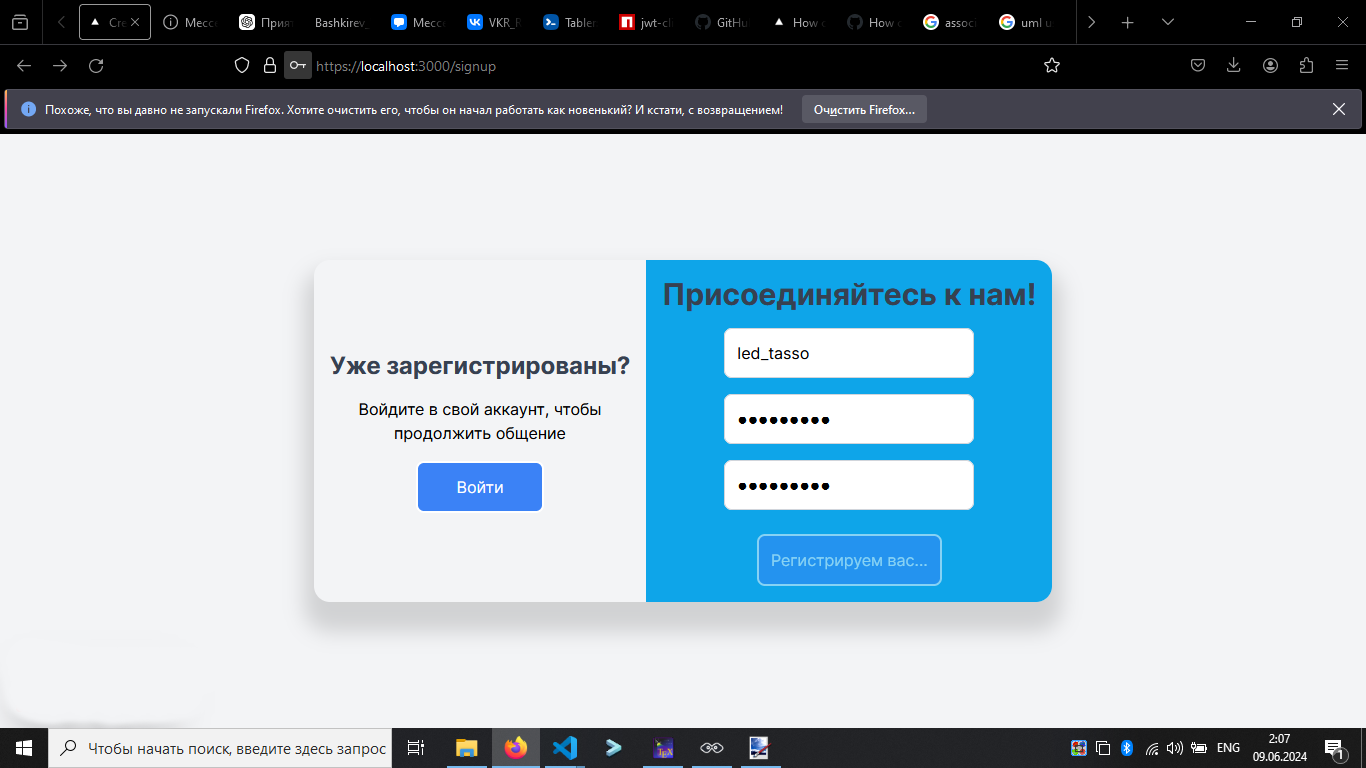
\includegraphics[width=1\linewidth]{signup_test1}}
	\caption{Процесс регистрации пользователя}
	\label{signup_test1:image}
\end{figure}

\begin{figure}[H]
	\center{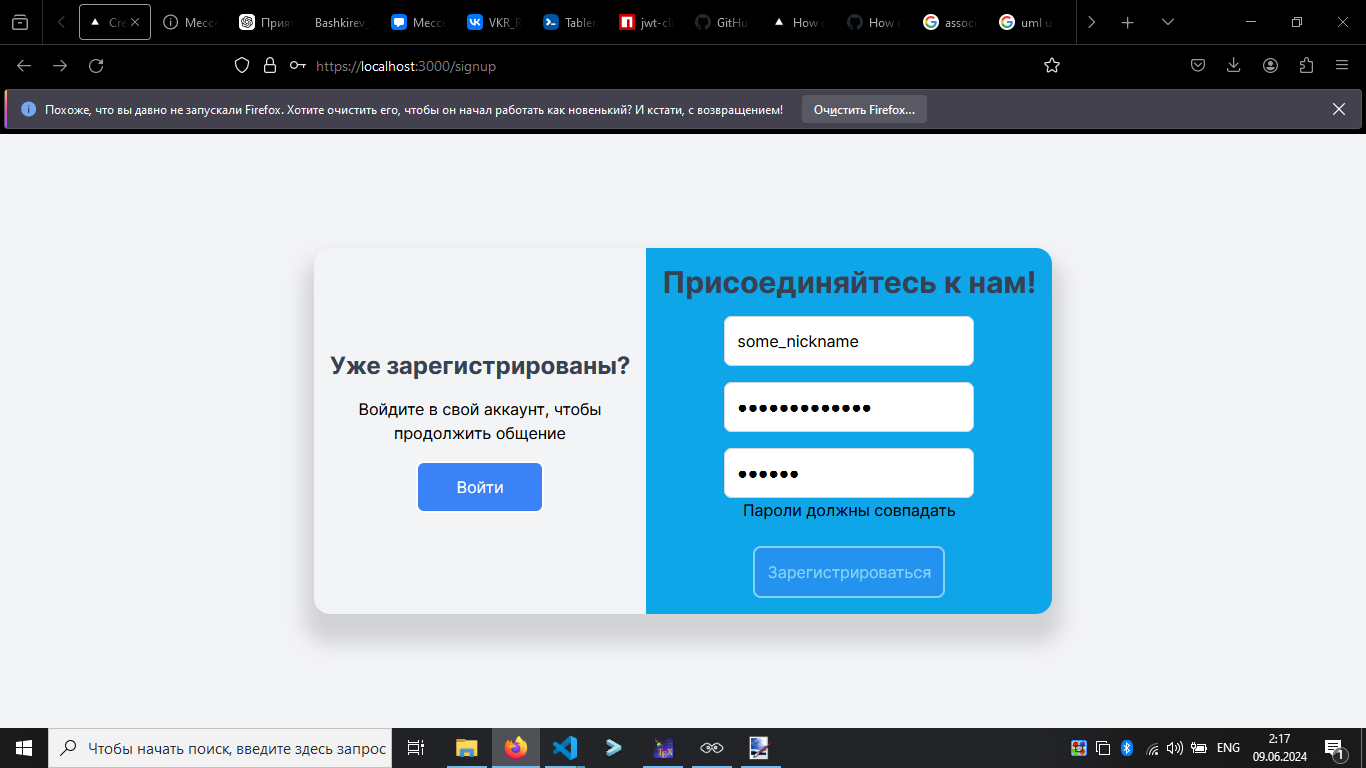
\includegraphics[width=1\linewidth]{signup_test2}}
	\caption{Попытка регистрации с неверными данными}
	\label{signup_test2:image}
\end{figure}

\begin{figure}[H]
	\center{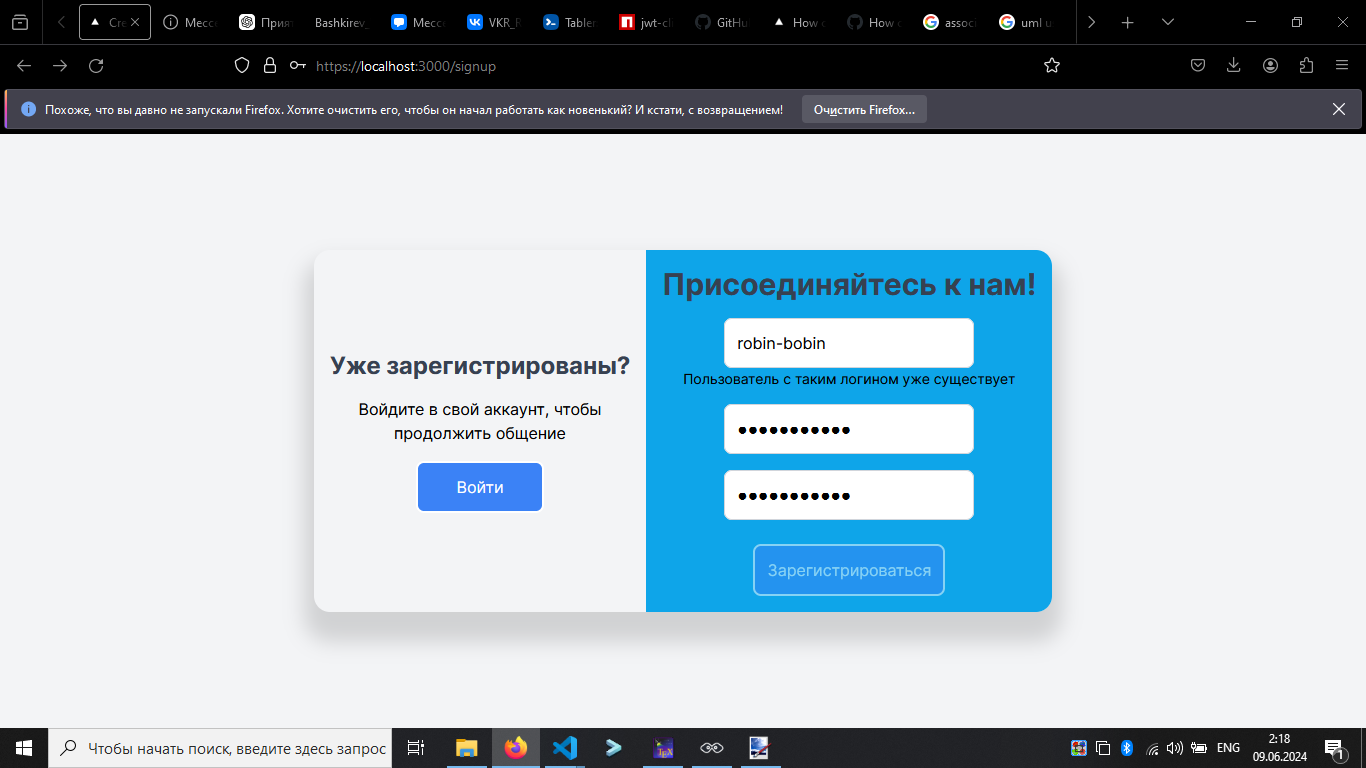
\includegraphics[width=1\linewidth]{signup_test3}}
	\caption{Попытка регистрациии с занятым логином}
	\label{signup_test3:image}
\end{figure}

После регистрации пользователь попадает на главную страницу. Результат представлен на рисунке \ref{signup_test4:image}.

\begin{figure}[H]
	\center{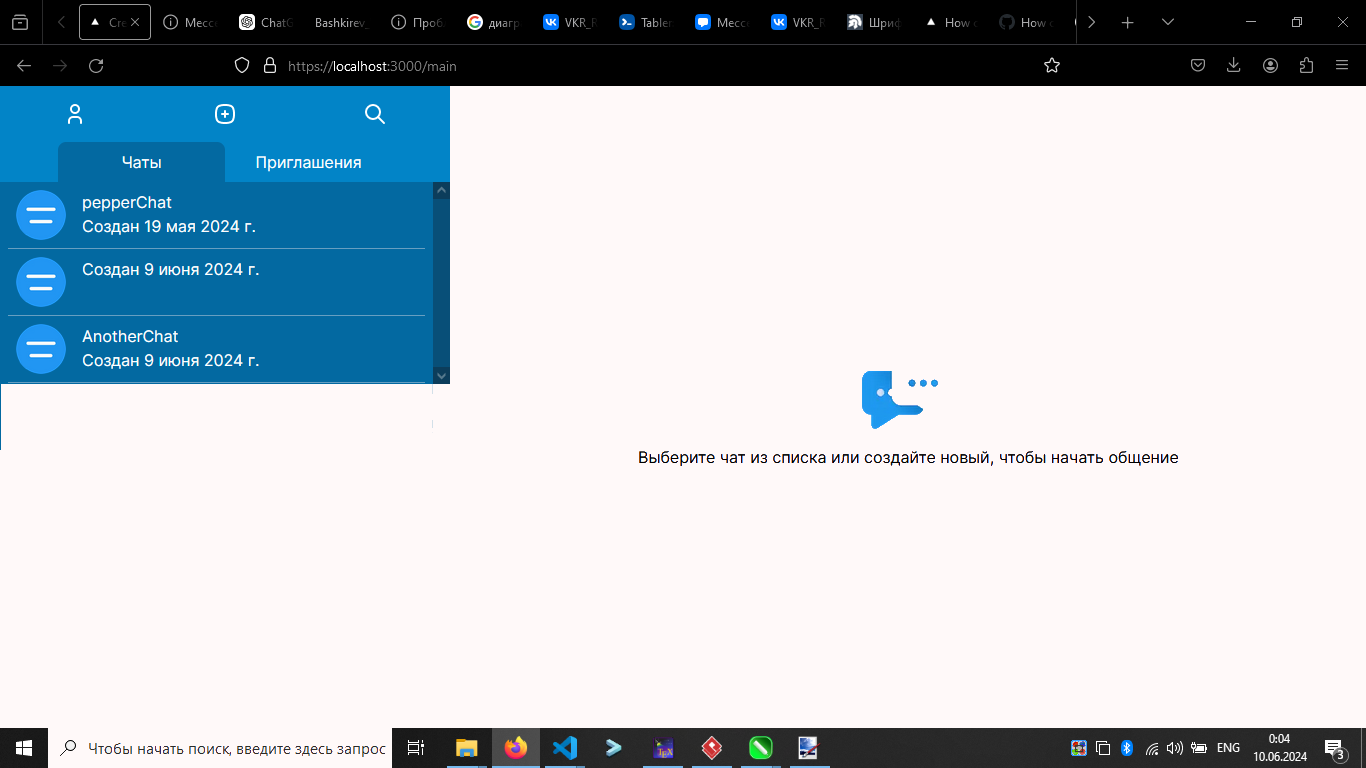
\includegraphics[width=1\linewidth]{signup_test4}}
	\caption{Переадресация на главную страницу приложения}
	\label{signup_test4:image}
\end{figure}

Приозведем тестирование функционала изменения личных данных в кабинете пользователя. Для этого попробуем изменить логин пользователя. Результаты тестирования представлены на рисунках \ref{cabinet_test1:image} и \ref{cabinet_test1:image}.


\begin{figure}[H]
	\center{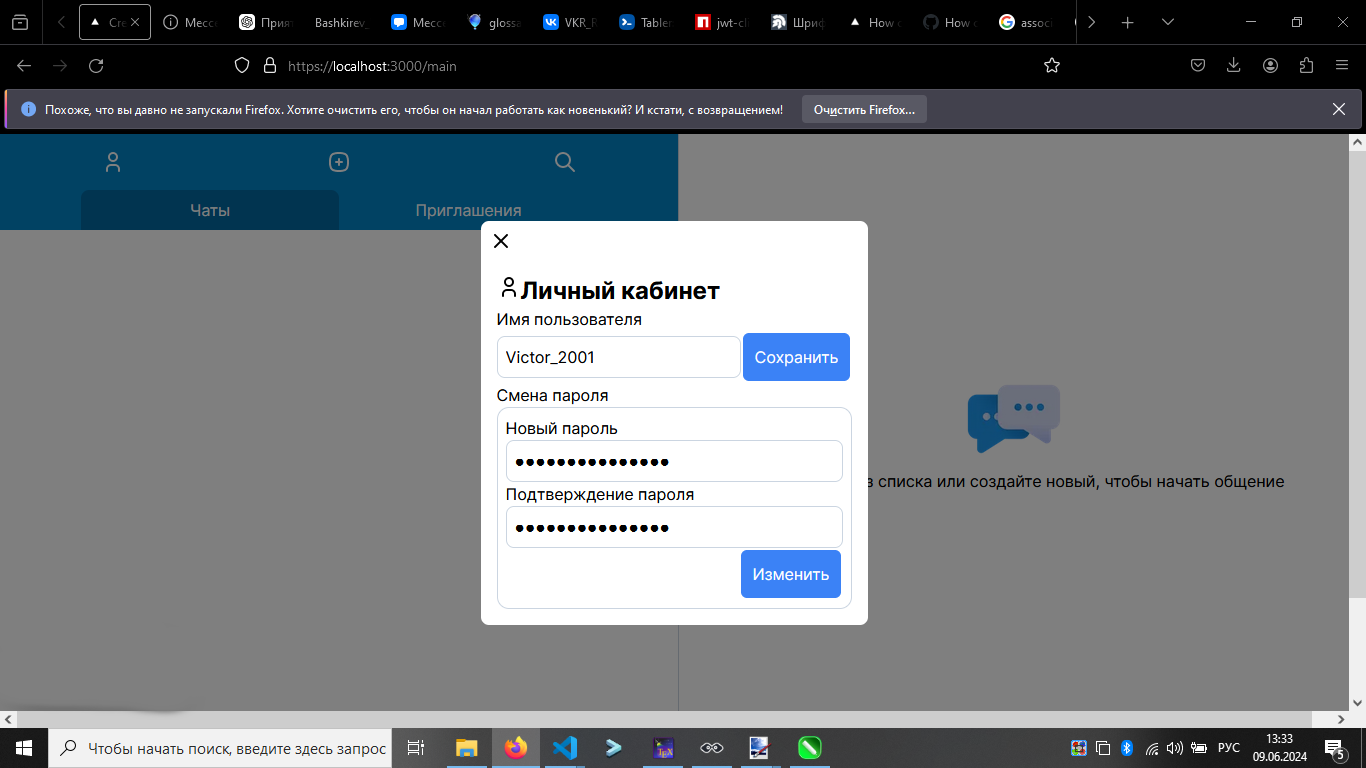
\includegraphics[width=1\linewidth]{cabinet_test1}}
	\caption{Личный кабинет пользователя с исходным логином}
	\label{cabinet_test1:image}
\end{figure}

\begin{figure}[H]
	\center{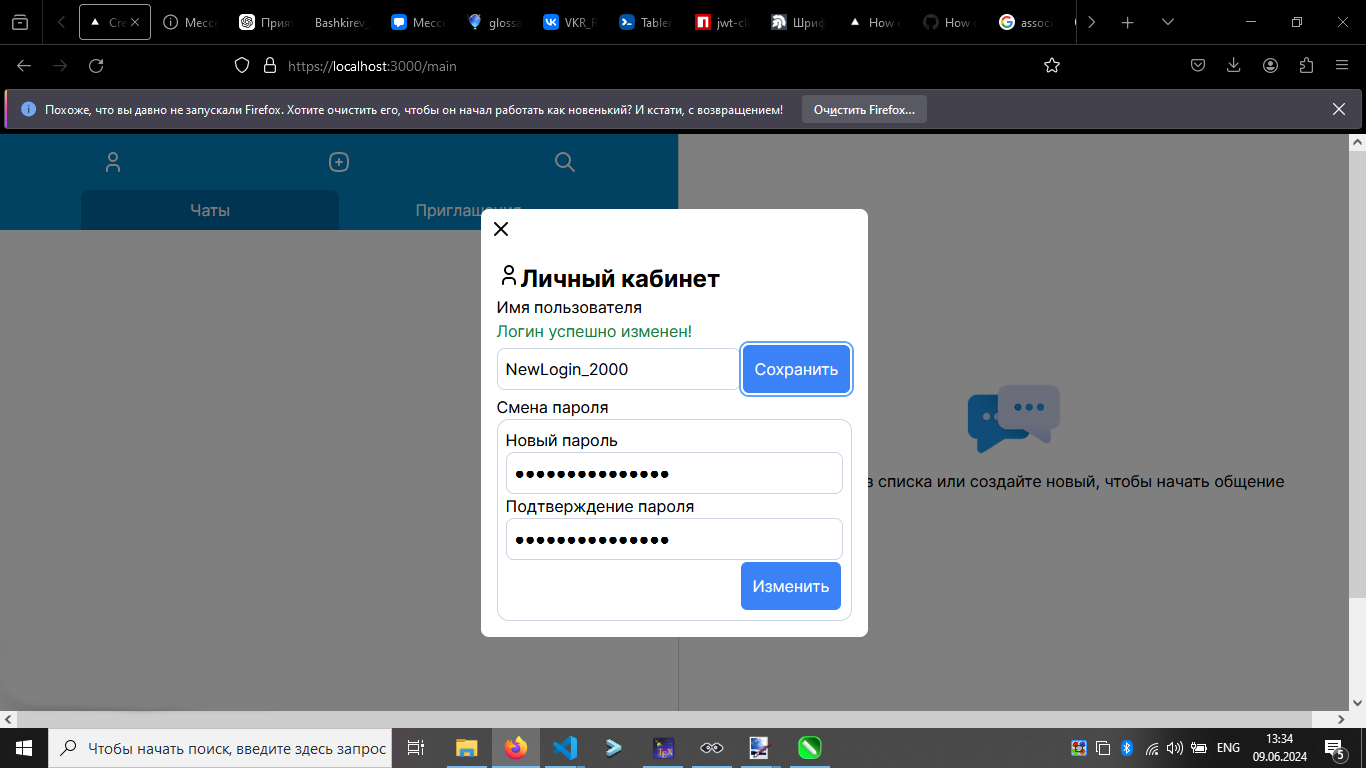
\includegraphics[width=1\linewidth]{cabinet_test2}}
	\caption{Результат изменения логина}
	\label{cabinet_test2:image}
\end{figure}

Далее протестируем функционал создания нового чата. Результаты тестов представлены на рисунках.

\begin{figure}[H]
	\center{\includegraphics[width=1\linewidth]{newChat_test1}}
	\caption{Ввод имени нового чата}
	\label{newChat_test1:image}
\end{figure}

\begin{figure}[H]
	\center{\includegraphics[width=1\linewidth]{newChat_test2}}
	\caption{Сообщение о успешном создании нового чата}
	\label{newChat_test2:image}
\end{figure}

\begin{figure}[H]
	\center{\includegraphics[width=1\linewidth]{newChat_test3}}
	\caption{Новый чат в списке чатов пользователя}
	\label{newChat_test3:image}
\end{figure}

Произведем тестирование функционала отправки сообщения. Для этого введем в поле ввода сообщения его текст и нажмем кнопку "<Отправить">. Результаты тестирования представлен на рисунках.

\begin{figure}[H]
	\center{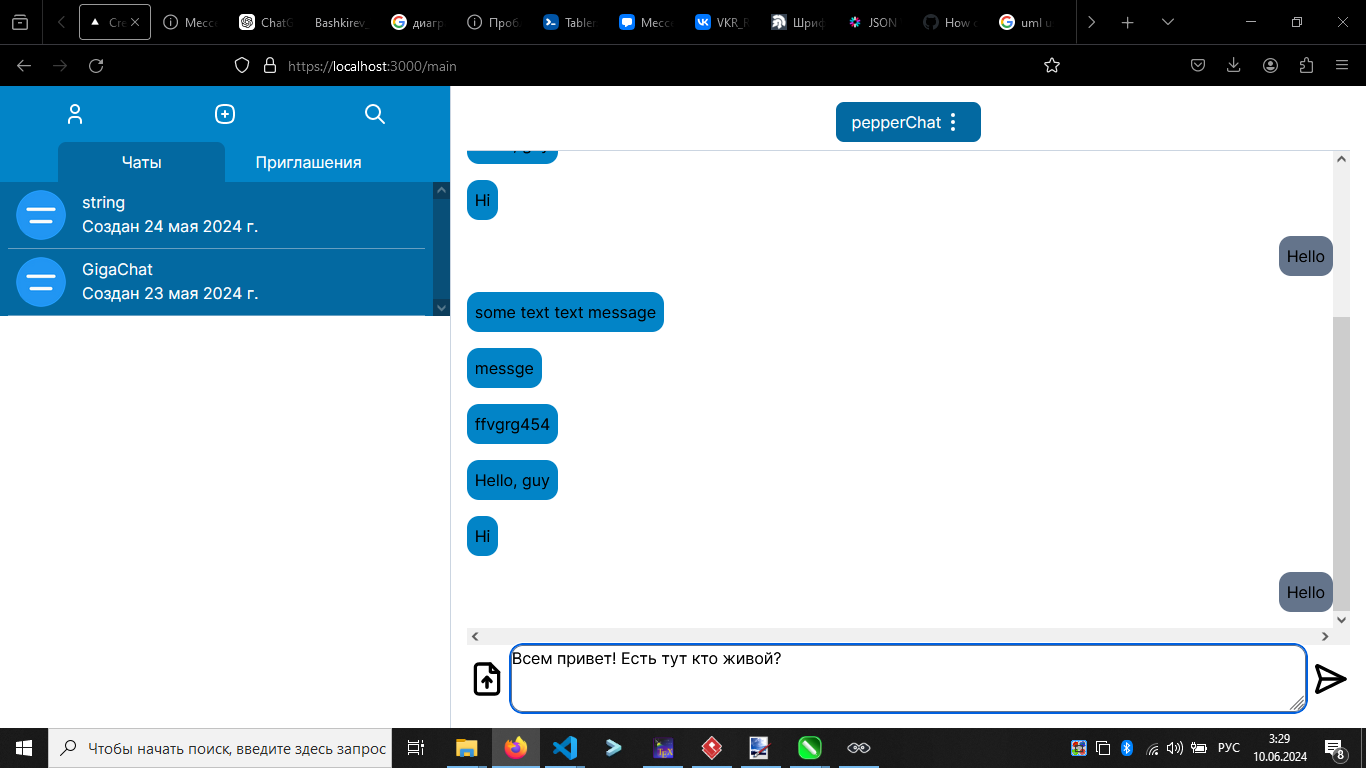
\includegraphics[width=1\linewidth]{newmessage_test1}}
	\caption{Вввод и отправка нового сообщения}
	\label{newmessage_test1:image}
\end{figure}

\begin{figure}[H]
	\center{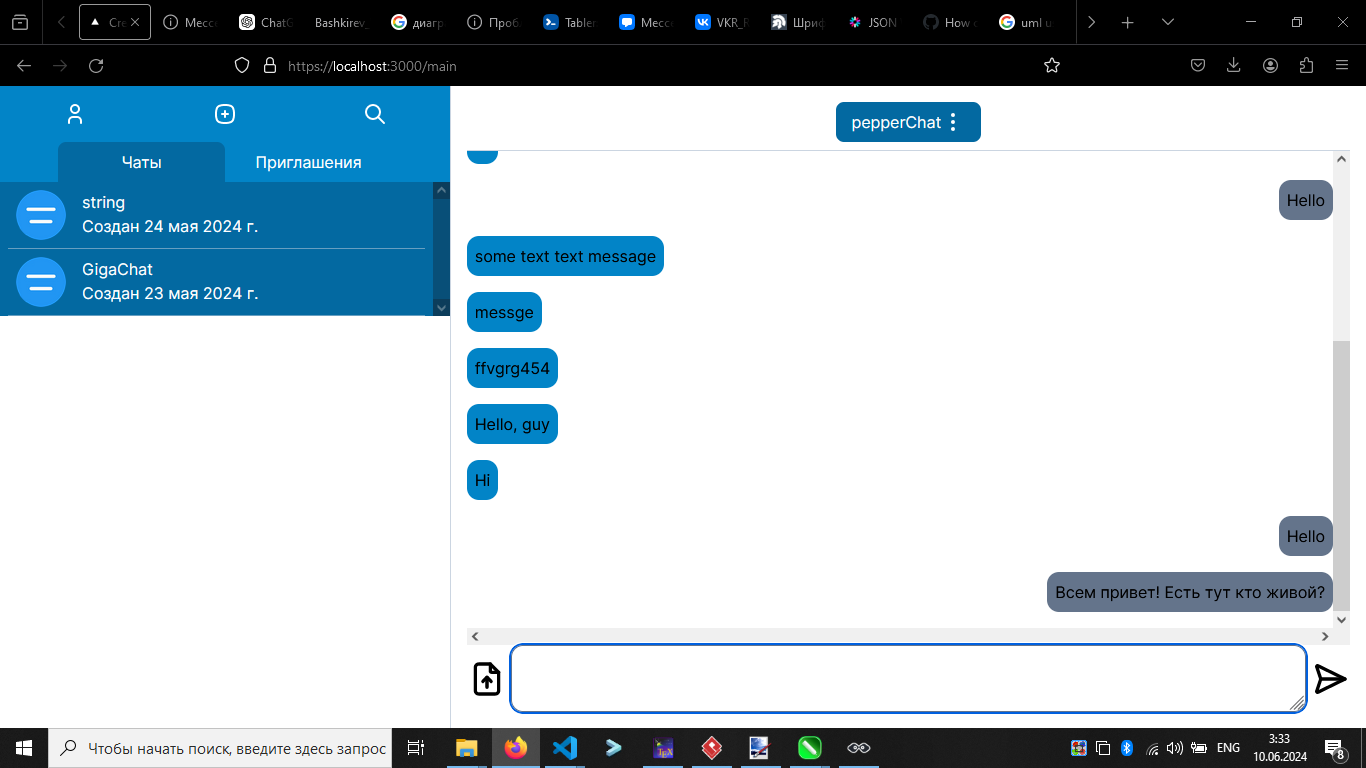
\includegraphics[width=1\linewidth]{newmessage_test2}}
	\caption{Результат отправки сообщения}
	\label{newmessage_test2:image}
\end{figure}

Произведем тестирование функционала входа в приложение. Для этого на странице входа в соответствующие поля необходимо ввести логин и пароль и нажать кнопку "<Войти">. Результаты тестирования представлены на рисунках.

\begin{figure}[H]
	\center{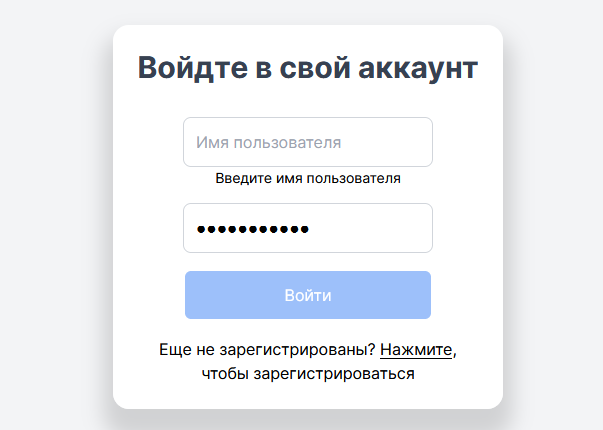
\includegraphics[width=1\linewidth]{signin_test1}}
	\caption{Попытка входа с неверными данными}
	\label{signin_test1:image}
\end{figure}

\begin{figure}[H]
	\center{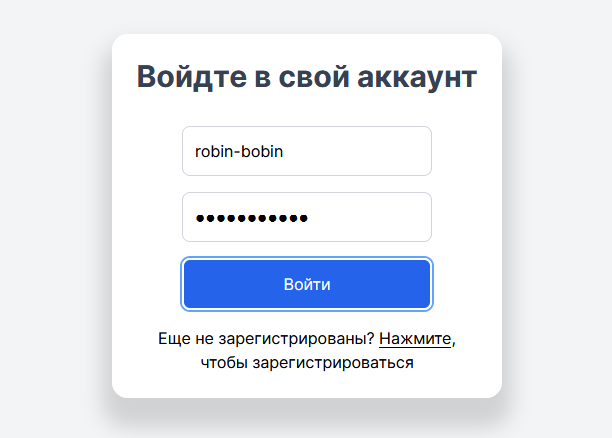
\includegraphics[width=1\linewidth]{signin_test2}}
	\caption{Ввод данных пользователя}
	\label{signin_test2:image}
\end{figure}

\begin{figure}[H]
	\center{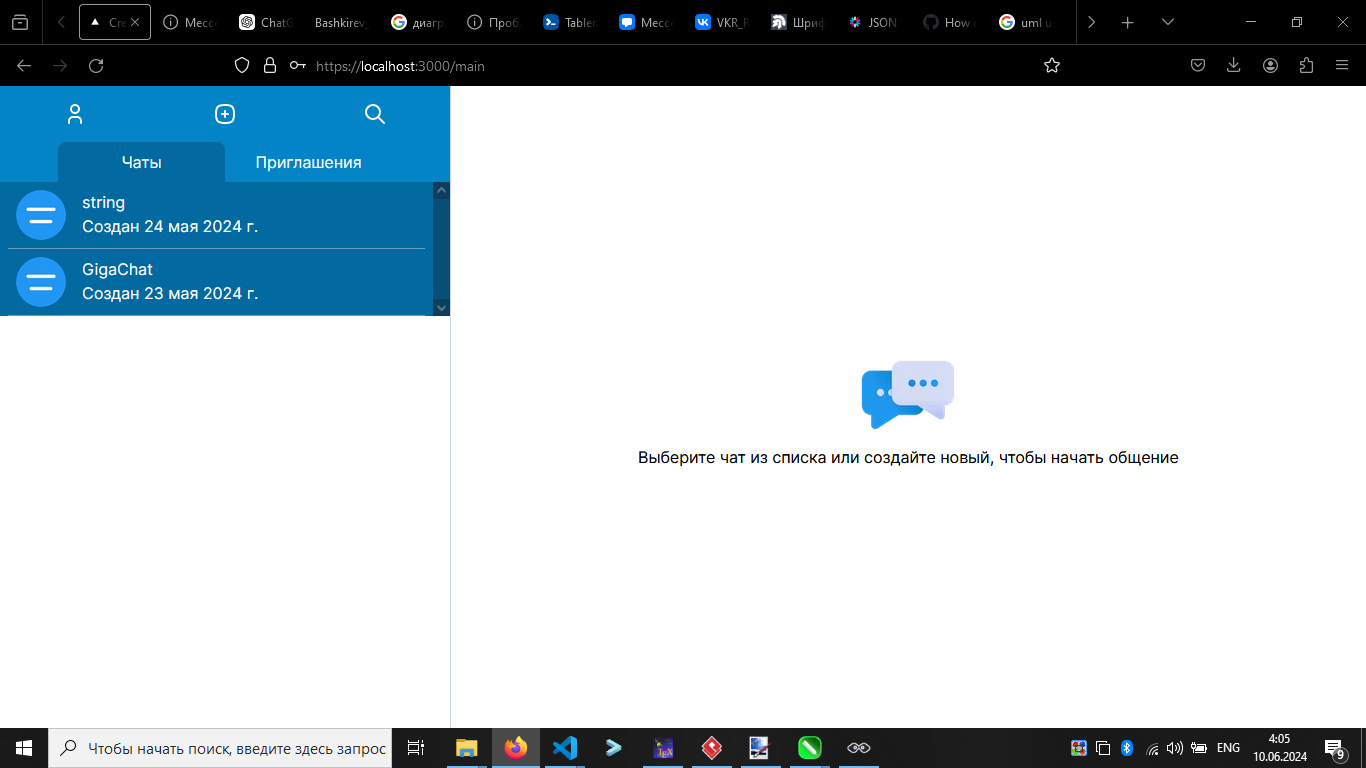
\includegraphics[width=1\linewidth]{signin_test3}}
	\caption{Главная страница после входа в приложение}
	\label{signin_test3:image}
\end{figure}